\documentclass{book} 

\usepackage{indentfirst}
\usepackage{booktabs}
\usepackage{multirow}
\usepackage{framed}
\usepackage{graphicx}
\usepackage{float}
\begin{document}
\title{Final Project Report}
\author{Zhou Litao, Fang Shaoheng, Dong Shiwen, Yang Hongbo}
\date{\today}


\maketitle


\tableofcontents





\frontmatter
\chapter {Preface}

A brief introduction to our team and our project. .... 

Introduce all the functions of our pages in a list. 

\paragraph{index.php}..... function A completed by xxx

\paragraph{search pages}.....

\paragraph{affiliation pages}.....

.....

Show how we use github to help with our work.

Give thanks to our instructors and the codes we've copied (expected to give specific links)


\mainmatter
\chapter {Enrich the Contents}

\section {Paper \& Conference Pages}

yhb

\subsection{Description}

\subsection{Solution}

\paragraph{point 1}

\paragraph{point 2}

\subsection{Source Codes}

\begin{minipage}[r]{15em}
\begin{verbatim}

short code example

\end{verbatim}
\end{minipage}

\subsection{Explanation}

\subsection{Demonstration}

\begin{figure}[H]
\centering

\includegraphics[height=4.0cm,width=4.0cm]{img/yhb_1.jpg}
\caption{IMG EXAMPLE}
\end{figure}

\section {Affiliation Pages}

We'd like to add a new series of pages to show affiliation information to users. Since we didn't do any previous work about affiliation information in the previous labs except that the affiliation table was input into the database, we have to write new SQL commands in search of affiliation information, and echo them out on the pages. The paper table and charts on other pages can be of help in showing the affiliation related information. Also, we have already got the author table written in the paper information page. Generally speaking, the work here is to collect the affiliation data and arrange them in order on the pages.


\subsection {Description}

The final version of the affiliation section include 3 concrete pages. On the affiliation\_info.php page, we will give three numbers on top of the page, counting all the authors, papers, and references in the affiliation. Then the authors in the affiliation will be listed below, together with their own affiliation information (hyper-links included) and number of publications. Affiliation\_paper.php shows all the papers related to the affiliation. The affiliation\_charts.php, where three charts are displayed, will be reported in detail in the Statistical Graph Section.

In fact, for the same function to be displayed on the page, we did two versions of code to implement them. The first one was very basic, just like those in the paper/author/search pages. However, since all the affiliation data are selected from the big paper\_author\_affiliation table, the first version didn't perform well in loading speed. Our optimization will be introduced in the Optimization Chapter.


\subsection{Solution \& Codes}

\subsubsection {Total Counts}
On top of every affiliation page, we've counted all the authors, papers and references concerned. For authors and papers, we can directly count them in the paper\_author\_affiliation table. For references, we first select the papers and then join the selected results to the paper\_reference table in order to count the results. The MySQL commands are listed below.

\begin{figure}[H]
\centering
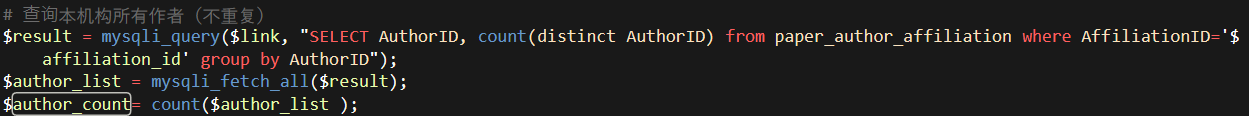
\includegraphics{img/zlt_aff_authorcount.png}
\caption{Count Author Commands}
\end{figure}
\begin{figure}[H]
\centering
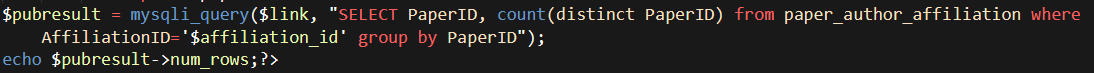
\includegraphics{img/zlt_aff_papercount.png}
\caption{Count Paper Commands}
\end{figure}
\begin{figure}[H]
\centering
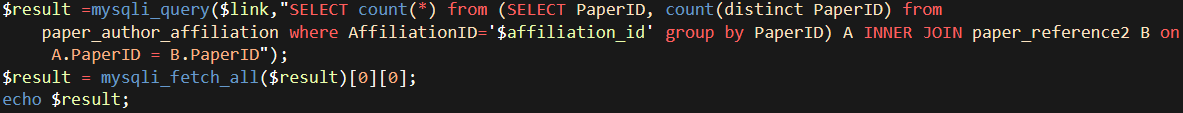
\includegraphics{img/zlt_aff_refcount.png}
\caption{Count Reference Commands}
\end{figure}

Note that we've use some MySQL techniques such as DISTINCT (eliminate overlapping results) and GROUP BY (perform data counting job) in order to implement our function.

For the data display in our page, our template has already provided a well designed data container in CSS, which can list different numbers in a row, with even width. We can simply apply this pre-defined class in a way demonstrated below.

\begin{figure}[H]
\centering
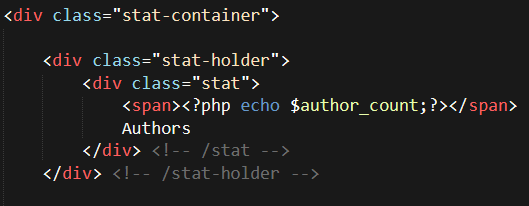
\includegraphics{img/zlt_aff_countdisplay.png}
\caption{Use Pre-defined Class to Display Numbers}
\end{figure}


\subsubsection{Authors List}

The author we've found based on the given affiliaiton may have more than one affiliation where he publishes his paper. All of the data related to this problem can be selected from the paper\_author\_affiliation table. As a result, our first design is to first sort out all the authors where the affiliation column fits, then we search the table again for affiliation information based on the author's id, which can be realized by looping through the author array in PHP. The first step has been done when we count the authors, so we simply skip the first step, call the author selecting result in the counting section, and make further searching based on the previous result. During the second step, we've also used DISTINCT \& GROUP BY techniques in order to get the author's affiliation data right and unrepeated.








\chapter{Leaf Turning}

dsw

\section{Version I: by PHP parameters}

\subsection{Description}

\subsection{Solution}

\paragraph{point 1}

\paragraph{point 2}

\subsection{Source Codes}

\begin{minipage}[r]{15em}
\begin{verbatim}

short code example

\end{verbatim}
\end{minipage}

\subsection{Explanation}

\subsection{Demonstration}

\begin{figure}[H]
\centering

\includegraphics[height=4.0cm,width=4.0cm]{img/dsw_1.jpg}
\caption{IMG EXAMPLE}
\end{figure}


\section{Version II: by jQuery}



\chapter {Integrated Searching Bar}

fsh


\chapter {Data Visualization}


\section {Statistical Graph}

fsh

\subsection{Description}

\subsection{Solution}

\paragraph{point 1}

\paragraph{point 2}

\subsection{Source Codes}

\begin{minipage}[r]{15em}
\begin{verbatim}

short code example

\end{verbatim}
\end{minipage}

\subsection{Explanation}

\subsection{Demonstration}

\begin{figure}[H]
\centering

\includegraphics[height=4.0cm,width=4.0cm]{img/fsh_1.jpg}
\caption{IMG EXAMPLE}
\end{figure}



\section {Paper Relation Graph}

zlt

\subsection{Description}

\subsection{Solution}

\paragraph{point 1}

\paragraph{point 2}

\subsection{Source Codes}

\begin{minipage}[r]{15em}
\begin{verbatim}

short code example

\end{verbatim}
\end{minipage}

\subsection{Explanation}

\subsection{Demonstration}


\section{Big Charts using Gephi}

gephi yhb



\chapter {Beautify the Pages}

\section {Index Beautification}

fsh

\section {Information Pages Beautification}

zlt


\chapter {MySQL Optimization in Affiliation Pages}

zlt

\end{document}
